% ---------------------------------------------------------------------------
% Visualisation section for the final write-up.
% Paste this file into the report or \input{} it. Required in the preamble:
%   \usepackage{graphicx,booktabs,amsmath,amssymb,xcolor}
%   \usepackage{tikz}
%   \usetikzlibrary{arrows.meta,positioning}
% Optional: \usepackage{flafter} keeps Figure 1 from floating above the heading.
% Figures: images are referenced as figures/viz_*. Copy writeup/latex/figures/
% next to the report's main .tex, or add the folder that contains figures/ to
% \graphicspath, e.g. \graphicspath{{writeup/latex/}}. They are built by
% make_figures.py. Citations: add viz_refs.bib to the report's bibliography.
% Status colours are those of the UI. Demote \section/\subsection if the section
% sits deeper in the report's hierarchy.
% ---------------------------------------------------------------------------
\definecolor{vizclear}{HTML}{1EA6AC}
\definecolor{viznear}{HTML}{E0B000}   % UI yellow #FFD24A, darkened for print
\definecolor{vizcrit}{HTML}{EF5255}
\definecolor{vizink}{HTML}{22303C}
\definecolor{vizmuted}{HTML}{6B7785}

\tikzset{
  vizbadge/.style={circle, fill=white, draw=black, line width=0.5pt,
    inner sep=0pt, minimum size=11pt, font=\sffamily\bfseries\scriptsize},
  vizlead/.style={white, line width=0.7pt},
}
% \vizbadge{n}{badge x,y}{target x,y}: numbered callout on a screenshot,
% coordinates as fractions of the image width and height (origin bottom left).
\newcommand{\vizbadge}[3]{%
  \draw[vizlead] (#2) -- (#3);
  \node[vizbadge] at (#2) {#1};}

\section{Visualisation: the depth-guidance workstation}\label{sec:viz}

The tracker delivers the 3D positions of both forceps jaw tips for each
microscope frame it can reconstruct (about 15\,Hz live). The workstation
(\texttt{services/viz}, React and three.js in the browser, fed over a WebSocket)
turns these positions into one quantity, the \emph{clearance} of the instrument
above the retina. It is a proof of concept for training on the Eyesi simulator,
not a medical device. Its readers are the trainee, who glances at it between
looks into the oculars, and an instructor watching the same screen live. The design follows one rule: the most important answer must be readable first and at a glance, with
detail behind it. We reduced the task to three questions, which loosely map onto
the perception, comprehension and projection levels of situation
awareness~\cite{endsley1995}:
\textbf{Q1}~How close is the instrument to the retina?
\textbf{Q2}~Which of the two tips is closer?
\textbf{Q3}~Is it getting closer?

\begin{figure*}[tp]
  \centering
  \begin{tikzpicture}
    \node[anchor=south west, inner sep=0] (img)
      {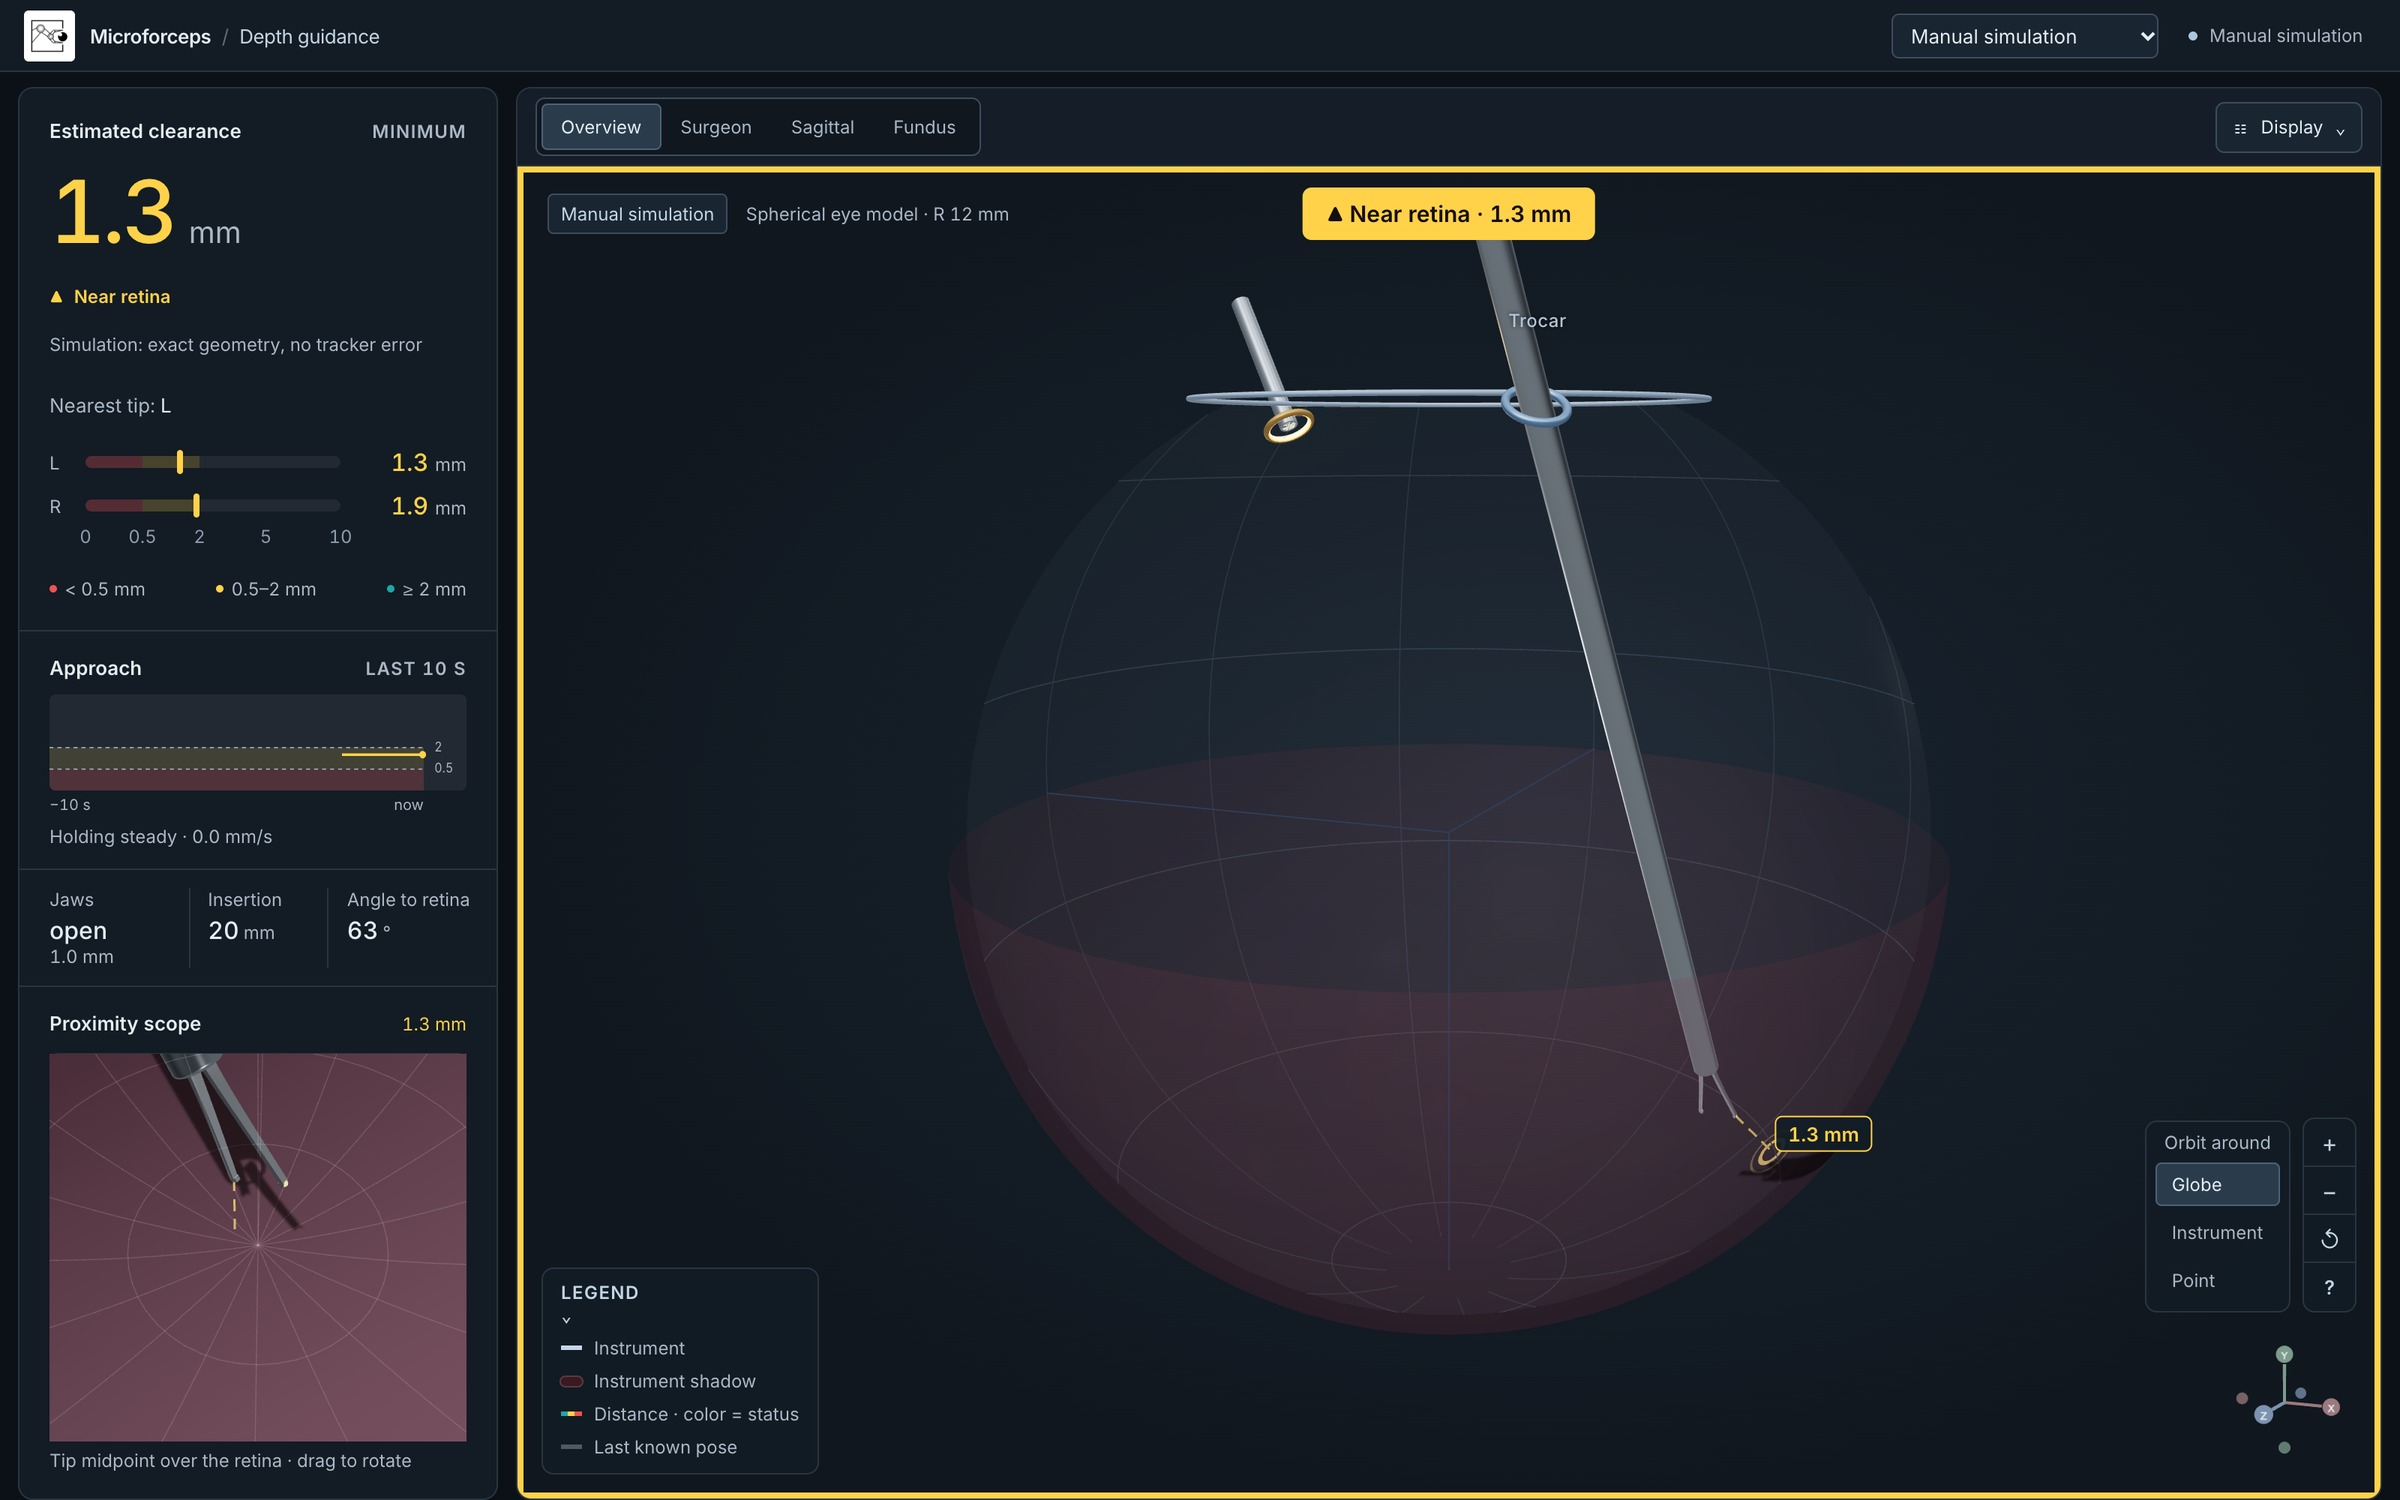
\includegraphics[width=\textwidth]{figures/viz_overview.jpg}};
    % magnified inset of the tip region, drawn in an empty part of the scene
    \begin{scope}[x={(img.south east)}, y={(img.north west)}]
      \draw[white, densely dashed, line width=0.5pt] (0.690,0.192) rectangle (0.795,0.304);
      \node[anchor=north west, inner sep=0, draw=white, line width=0.8pt] (inset)
        at (0.235,0.800)
        {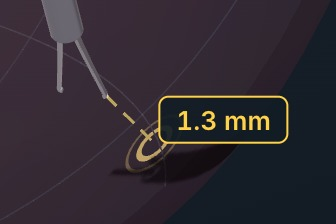
\includegraphics[width=0.18\textwidth]{figures/viz_overview_tip.jpg}};
      \draw[white, densely dashed, line width=0.4pt] (inset.south east) -- (0.690,0.304);
    \end{scope}
    \begin{scope}[x={(img.south east)}, y={(img.north west)}]
      \vizbadge{1}{0.150,0.868}{0.105,0.858}
      \vizbadge{2}{0.192,0.770}{0.178,0.770}
      \vizbadge{3}{0.125,0.730}{0.075,0.730}
      \vizbadge{4}{0.165,0.442}{0.145,0.505}
      \vizbadge{5}{0.215,0.375}{0.200,0.375}
      \vizbadge{6}{0.120,0.318}{0.120,0.290}
      \vizbadge{7}{0.687,0.858}{0.665,0.858}
      \vizbadge{8}{0.432,0.700}{0.415,0.700}
      \vizbadge{9}{0.423,0.916}{0.409,0.916}
      \vizbadge{10}{0.435,0.858}{0.421,0.858}
      \vizbadge{11}{0.772,0.976}{0.788,0.976}
    \end{scope}
  \end{tikzpicture}
  \caption{The workstation with the forceps close to the retina and the left jaw
  nearer (pose set by hand in the simulation mode; all screenshots are of the
  running application). Left column, read top to bottom from coarse to fine:
  \textbf{1}~estimated clearance of the nearer tip with status word and symbol
  (Q1); \textbf{2}~accuracy note; \textbf{3}~nearest tip and one depth bar per
  tip (Q2); \textbf{4}~approach trend of the last 10\,s with motion word and rate
  (Q3); \textbf{5}~instrument context (jaws, insertion, angle);
  \textbf{6}~proximity scope, a magnified view of the retina below the jaw
  midpoint with a drop line from the nearer tip. 3D view: \textbf{7}~scene alarm (frame and
  banner); \textbf{8}~instrument shadow, drop line, landing reticle and distance
  label (inset: dashed region, magnified; the short instrument on the left is
  the light pipe); \textbf{9}~view presets; \textbf{10}~model assumption (spherical eye,
  $R = 12$\,mm); \textbf{11}~data source and connection.}
  \label{fig:viz-overview}
\end{figure*}

\subsection{Layout and encoding}\label{sec:viz-layout}

Figure~\ref{fig:viz-overview} shows the screen. The left column answers the three
questions in reading order; the 3D view on the right provides spatial context and
repeats the alarm, but never holds the only copy of a number.

\paragraph{Q1: one number.} The clearance of each tip is its radial distance to a
sphere of radius 12\,mm, $d = \max(0,\,12\,\text{mm} - \lVert\mathbf{p}_\text{tip}\rVert)$
with $\mathbf{p}_\text{tip}$ measured from the eye centre, and the large number shows the minimum over both tips. It has one decimal and is rounded \emph{down}. Two decimals would
claim a resolution about 60 times finer than the tracker's median height error of
0.63\,mm, while a reported value should carry no more digits than its
uncertainty justifies~\cite{gum2008}; whole millimetres would hide useful distinctions around the 0.5\,mm
threshold. Rounding down keeps the number from ever
exceeding the estimate and makes it agree with the instantaneous level at a
threshold (0.46\,mm reads ``0.4'' next to Critical).

\paragraph{Status levels.} Three provisional training
levels, \emph{Clear} ($\geq 2$\,mm), \emph{Near retina} (0.5--2\,mm) and
\emph{Critical proximity} ($< 0.5$\,mm), are each coded three times: as colour,
as word and as symbol ($\bullet$, $\blacktriangle$, $\blacksquare$). The level can
therefore be read without colour. The palette (teal, yellow, red) moves ``safe'' from green to teal,
away from the red--green confusion axis~\cite{wong2011}; yellow also differs in
lightness, while teal and red differ mainly in hue, which is why word and symbol
are needed. Under simulated full
deuteranopia~\cite{machado2009}, the colour difference between safe and danger
rises from $\Delta E_{00} = 7.8$ (earlier green/amber/red palette) to 35.3. In simulation mode, as in Figure~\ref{fig:viz-overview}, the
accuracy note (2) states that the geometry is exact. In live mode it summarises
the simulator recordings for the level currently shown (Figure~\ref{fig:viz-states}b): for
Critical and Near, the 10th--90th percentile of the logged midpoint clearance
among measured frames at that displayed level; for Clear, the median bias.

\paragraph{Q2 and Q3.} The two depth bars place each tip on a square-root scale
from 0 to 10\,mm, so the decision-relevant first 2\,mm take 45\,\% of the bar
instead of 20\,\% on a linear scale. ``Nearest tip: L / R / L\,$\approx$\,R'' names
the nearer jaw. A tie band (enter below 0.10\,mm, leave above 0.15\,mm)
absorbs noise between the tips; adding a 500\,ms dwell cut label changes from 71
to 10 per minute in the replay. The approach trend uses the same
scale and threshold lines as the bars, so a level reads the same in both. Because
the slope on a square-root axis is not the velocity, the rate is printed as a
number next to a motion word (\emph{Approaching}, \emph{Holding steady},
\emph{Retracting}). An earlier time-to-contact countdown was removed: it divided a
biased distance by a noisy velocity and looked like a measurement.

\paragraph{3D cues.} The overview alone cannot show sub-millimetre gaps. Three cues
make depth visible in 3D (inset and scope in Figure~\ref{fig:viz-overview}): a shadow cast
from the light pipe (its position is fixed by the calibration), a strong cue for
motion in depth~\cite{kersten1997}; a drop line from the nearer tip to the
retina; and a reticle where that line meets the retina. Like the ``Nearest tip''
label, the drop line follows the stabilised nearer-tip selection (the midpoint
for a tie), while the number stays the instantaneous minimum. The proximity
scope (6) is a second, linked view~\cite{roberts2007} of the retina directly
below the jaw midpoint. It turns on below 5\,mm and keeps a fixed place in the layout, so
the screen does not rearrange at the moment of highest risk.

\begin{figure}[tbp]
  \centering
  \resizebox{\linewidth}{!}{%
  \begin{tikzpicture}[lbl/.style={anchor=south east, inner sep=3pt,
      text=white, font=\sffamily\bfseries\small}]
    \node[anchor=north west, inner sep=0] (a) at (0,0)
      {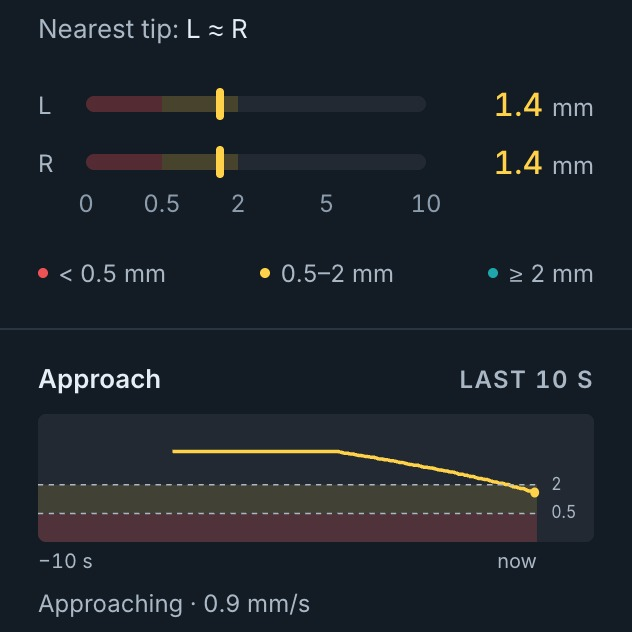
\includegraphics[height=84mm]{figures/viz_card_trend.jpg}};
    \node[anchor=north west, inner sep=0] (b) at ([xshift=1mm]a.north east)
      {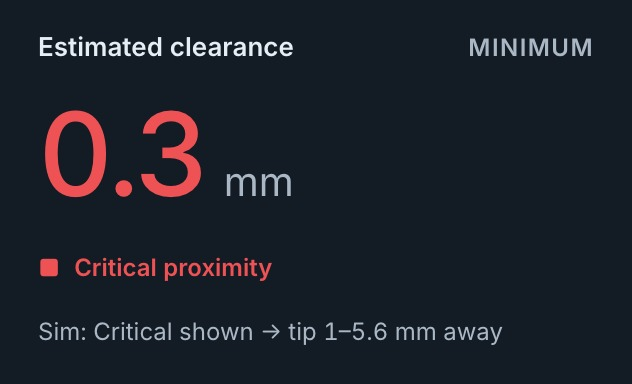
\includegraphics[height=27.33mm]{figures/viz_card_critical.jpg}};
    \node[anchor=north west, inner sep=0] (c) at ([yshift=-1mm]b.south west)
      {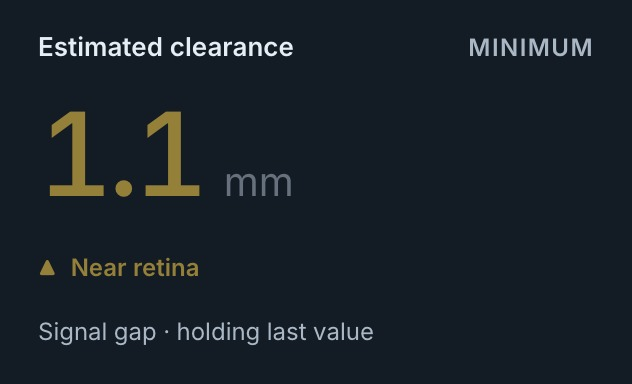
\includegraphics[height=27.33mm]{figures/viz_card_held.jpg}};
    \node[anchor=north west, inner sep=0] (d) at ([yshift=-1mm]c.south west)
      {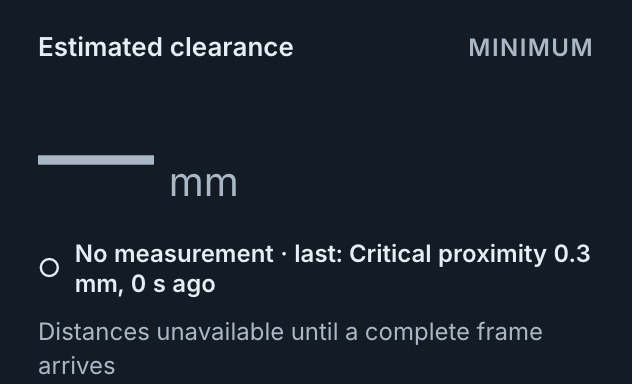
\includegraphics[height=27.33mm]{figures/viz_card_lost.jpg}};
    \node[lbl] at (a.south east) {(a)};
    \foreach \p in {b,c,d} \node[lbl, anchor=east] at (\p.east) {(\p)};
  \end{tikzpicture}}
  \caption{Left-column details, enlarged. (a) Nearest tip, depth bars, colour key and
  approach trend during a scripted approach in simulation mode (Q2, Q3); the
  whole trend line takes the colour of the current level. (b)--(d) The clearance card in live mode, driven by
  synthetic poses through a mocked WebSocket. In (b) the accuracy note reports
  that, when Critical was shown on the simulator recordings, the logged midpoint
  clearance was mostly 1--5.6\,mm (10th--90th percentile). (c) A short signal
  gap: the last value is held and dimmed. (d) Once 400\,ms have passed since the
  last measurement, the number disappears and the last reading is shown as
  history only; its ``s ago'' counter starts when this state appears, so it
  understates the age.}
  \label{fig:viz-states}
\end{figure}

\subsection{Alert logic}\label{sec:viz-alert}

A raw threshold applied frame by frame makes the status flicker. Measurement noise
makes it chatter at each threshold, and in the offline replay 26.5\,\% of frames
lack a reconstruction (including visibility and detection failures), so without
a grace period every gap would end an alarm. The workstation therefore separates
\emph{availability} (is there a current measurement?) from the \emph{distance
level} (how close is it?) and uses asymmetric rules (Figure~\ref{fig:viz-logic}).
Escalation is immediate: a warning must never arrive late because of filtering.
De-escalation requires the same safer candidate level, beyond a hysteresis margin
of 0.08\,mm (about twice the estimated per-sample noise), for 250\,ms of
uninterrupted measurements; a change of candidate or a gap restarts this dwell.
While a level is retained this way, the status reads, e.g., ``Critical proximity~$\cdot$~clearing''. Missing data is never shown as
safe. A missing or incomplete frame, or 200\,ms without any new frame, holds the
last values, dimmed and labelled ``Signal gap''. Once 400\,ms have passed since
the last valid measurement, the level is replaced by ``No measurement'' and the
last pose is shown as a faded ghost. A source whose timestamp stops advancing for
1.5\,s is marked stale. Figure~\ref{fig:viz-trace} shows the real pipeline code
processing a synthetic feed.

\begin{figure}[tbp]
  \centering
  \begin{tikzpicture}[
      font=\sffamily\footnotesize, >={Stealth[length=4pt]},
      lvl/.style={draw=#1, line width=1pt, rounded corners=2pt, fill=#1!10,
        minimum width=24mm, minimum height=7mm, align=center},
      av/.style={draw=vizmuted, rounded corners=2pt, fill=vizmuted!8,
        minimum width=20mm, minimum height=7mm, align=center},
      up/.style={->, vizink, line width=0.6pt},
      down/.style={->, vizink, line width=0.6pt, dashed},
      ret/.style={->, vizink, line width=0.6pt, dotted},
      lab/.style={font=\sffamily\scriptsize, text=vizink},
    ]
    % (a) distance level
    \node[anchor=west, font=\sffamily\bfseries\footnotesize] at (-1.6,1.55)
      {(a) Distance level, per tip};
    \node[lvl=vizclear] (clear) at (0,0) {$\bullet$ Clear\\[-1pt]\scriptsize $d \geq 2$};
    \node[lvl=viznear, right=13mm of clear] (near)
      {$\blacktriangle$ Near retina\\[-1pt]\scriptsize $0.5 \leq d < 2$};
    \node[lvl=vizcrit, right=13mm of near] (crit)
      {$\blacksquare$ Critical\\[-1pt]\scriptsize $d < 0.5$};
    \draw[up] ([yshift=1.5mm]clear.east) -- node[lab, above] {$d<2$} ([yshift=1.5mm]near.west);
    \draw[up] ([yshift=1.5mm]near.east) -- node[lab, above] {$d<0.5$} ([yshift=1.5mm]crit.west);
    \draw[down] ([yshift=-1.5mm]near.west) -- node[lab, below] {$\geq 2.08$} ([yshift=-1.5mm]clear.east);
    \draw[down] ([yshift=-1.5mm]crit.west) -- node[lab, below] {$\geq 0.58$} ([yshift=-1.5mm]near.east);
    \draw[up] (clear.north) to[out=30, in=150] node[lab, above] {$d<0.5$} (crit.north);
    \draw[down] (crit.south) to[out=-150, in=-30] node[lab, below] {$\geq 2.08$} (clear.south);
    \node[lab, align=left, anchor=north west] at ([yshift=-15mm]clear.south west)
      {\textbf{solid}: escalate on the first frame\\
       \textbf{dashed}: de-escalate after 250\,ms at the same candidate level\\
       box ranges are raw classification bands; levels can be skipped\\
       displayed level = more severe tip; distances in mm};
    % (b) availability
    \begin{scope}[yshift=-49mm]
      \node[anchor=west, font=\sffamily\bfseries\footnotesize] at (-1.6,1.05)
        {(b) Availability};
      \node[av] (trk) at (0,0) {Tracking\\[-1pt]\scriptsize live values};
      \node[av, right=11mm of trk] (held) {Held\\[-1pt]\scriptsize dimmed, level frozen};
      \node[av, right=16mm of held] (lost) {No measurement\\[-1pt]\scriptsize ghost pose, no alarm};
      \draw[up] ([yshift=1.5mm]trk.east) -- node[lab, above] {gap} ([yshift=1.5mm]held.west);
      \draw[up] (held) -- node[lab, above, align=center] {400\,ms after\\[-2pt]last valid} (lost);
      \draw[ret] ([yshift=-1.5mm]held.west) -- node[lab, below] {valid} ([yshift=-1.5mm]trk.east);
      \draw[ret] (lost.south) -- ++(0,-4mm) -| node[lab, pos=0.25, below] {next valid frame (level history reset)} (trk.south);
      \node[lab, anchor=north west] at ([yshift=-9mm]trk.south west)
        [align=left] {\textbf{gap}: missing or incomplete frame, or 200\,ms silence\\
         \textbf{dotted}: back to Tracking on the next valid frame};
    \end{scope}
  \end{tikzpicture}
  \caption{Two independent state axes. (a) Hysteresis and dwell act only on the
  way down. (b) Missing data is never read as safe: it holds the level for at
  most 400\,ms after the last valid measurement and then removes it. Not drawn: \emph{Stale} (source timestamp
  frozen for 1.5\,s) and \emph{Disconnected} (socket error, no grace).}
  \label{fig:viz-logic}
\end{figure}

\begin{figure}[tbp]
  \centering
  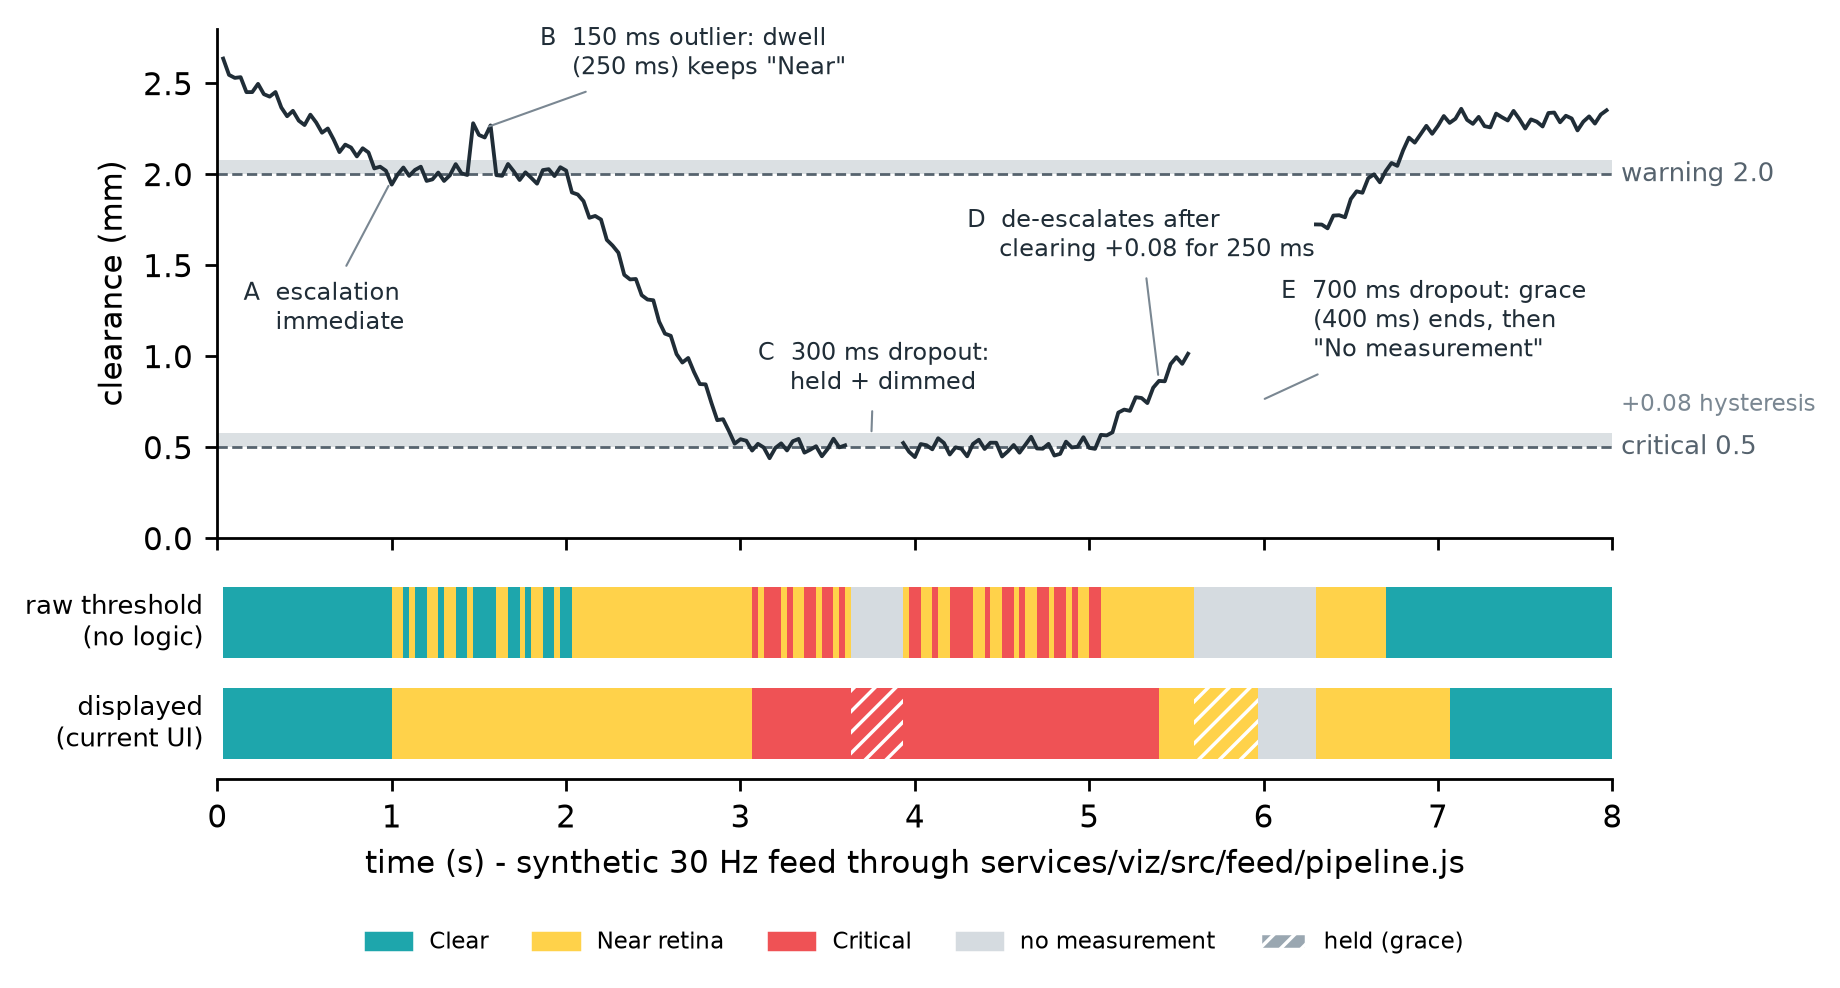
\includegraphics[width=\linewidth]{figures/viz_alert_trace.png}
  \caption{The pipeline code of the workstation processing a synthetic 30\,Hz
  feed. Top: input clearance with the thresholds and the 0.08\,mm hysteresis
  bands. Bottom: the raw threshold classification flickers; the displayed level
  escalates immediately (A), ignores a 150\,ms outlier (B), holds through a
  300\,ms dropout (C), releases after 250\,ms above the band (D) and, in a
  700\,ms dropout, shows ``No measurement'' once the 400\,ms grace has expired (E).}
  \label{fig:viz-trace}
\end{figure}

We replayed all three simulator recordings (11\,428 frames, 381\,s) through a
midpoint emulation of the previous and the current rules (the previous rules no
longer exist in code) and compared the result with the logged midpoint clearance,
our ground-truth proxy (Table~\ref{tab:viz-replay}). The new rules cut status
changes by almost two thirds and, by holding through its dropouts, recover the 0.63\,s of the one truly
critical episode that the previous rules missed (one episode, so no evidence of
detection accuracy). The cost is specificity: holding and
slower release make episodes longer, and most episodes are false to begin with.
Because the tracker mostly places the tip \emph{closer} than it is (80\,\% of valid reconstructions, median $-0.53$\,mm), the estimate often drops below 0.5\,mm while the tip
is still millimetres away, and Critical then stays until the release rules are
met. A second replay feeds both reconstructed tips through the UI pipeline
itself, with the same proxy. In it, the logged clearance at the onset of a Critical display
was 3.0\,mm (median), and only 3.2\,\% of the time Critical was shown had a logged
clearance below 0.5\,mm. We draw two
consequences in the design. First, the live Critical frame is steady red rather
than the flashing red that IEC~60601-1-8~\cite{iec60601-1-8} associates with
high-priority alarms, so that a mostly false red signal does not teach trainees
to ignore red~\cite{cvach2012}. There is also no audible alarm; this was a
project decision, and alarm fatigue is a further reason for it. Second, the
accuracy note states the problem openly instead of hiding it. The UI does not
correct the bias. It belongs to the orthographic camera model; on one recorded run, a perspective prototype with a camera fitted to that session
reduced the median height bias from $-0.50$ to $-0.11$\,mm.

\begin{table}[tbp]
  \centering
  \small
  \caption{Replay of the three simulator runs, emulating the rules on the
  reconstructed tip midpoint. Previous: 0.05\,mm hysteresis, no dwell, no grace;
  current: the rules of Figure~\ref{fig:viz-logic}. The replay through the actual
  UI pipeline (both tips, minimum shown) gives 54.9\,s of false critical time.}
  \label{tab:viz-replay}
  \begin{tabular}{@{}lrr@{}}
    \toprule
    metric (pooled over 381\,s) & previous & current \\
    \midrule
    status changes per minute (incl.\ availability) & 106.5 & 37.8 \\
    Near/Critical episodes ended by a dropout       & 126   & 39 \\
    missed critical time (s)                        & 0.63  & 0 \\
    false critical time (s)                         & 13.8  & 43.4 \\
    time shown as ``No measurement'' (\%)$^{a}$     & 26.5  & 15.6 \\
    \bottomrule
    \multicolumn{3}{@{}l}{\footnotesize $^{a}$ held values during the grace
      period count as shown.}
  \end{tabular}
\end{table}

\subsection{Data path and limitations}\label{sec:viz-limits}

The workstation does not average or filter the numeric clearances; levels change
only by the rules above, and the approach rate is smoothed (upstream, the live
detector smooths its 2D points with an exponential moving average, weight 0.5). The readout refreshes at most every 100\,ms, but a
change of level or availability is shown at once. Live instrument poses are interpolated between two measured poses (about 80\,ms behind, never extrapolated) to remove
stutter in the magnified scope. At the median approach speed within the last 3\,mm in the
recordings (0.53\,mm/s), this interpolation lag corresponds to 0.04\,mm, small compared with the
measurement error.

The design has been checked against recorded data, not against users. Three runs
by one user contain a single truly critical episode. The thresholds are
provisional, and hysteresis, dwell and grace were derived and evaluated on the
same data. Although the grace period removed most dropout-ended Near/Critical episodes
in the midpoint emulation, data loss still ends most Critical episodes in the UI replay
(32 of 58 observed endings followed grace expiry). In live operation, only
reconstruction failures arrive as gaps: after a detection dropout or a detector
stall, the stream server re-sends the last pose with a fresh send time, so the
screen shows a frozen but current-looking value. A capture timestamp from the
tracker would fix this. The recordings log only the tip midpoint, so the accuracy of Q2 (which tip is closer) is unmeasured. The 3D
position error (median 1.4--2.5\,mm) is larger than the height error, so the
reticle and the scope can look precise while being misplaced laterally. The next
steps are a heuristic evaluation and a small think-aloud study with trainees, and
a replay of new recordings once the perspective model is in place.
